\documentclass[]{article}

\usepackage{sectsty}

\usepackage[parfill]{parskip}

\usepackage{hyperref}

\usepackage[T1]{fontenc}

\usepackage{graphicx}

\usepackage[T1]{fontenc}

\sectionfont{\fontsize{10}{10}\selectfont}


\begin{document}


\author{
  Nikhil Chaturvedi\\
  \texttt{2013CS50291}
  \and
  Harman Kumar\\
  \texttt{2013CS10224}
}

\title{Game Of Thrones Wiki}
\maketitle



\section{Overall Design}

\begin{flushleft}

We present a complete database for the most popular TV series, Game of Thrones. We have over 1000 character stats and prediction about their survival based on popularity, number of dead relatives they have and how good their house is doing.

The system allows users to create password secured accounts in order in order to access the GOT Wiki. We also have a separate admin login which allows us to add new information to our databases using a form.\\

You can find the ER diagram of the project at the end of the document.

\end{flushleft} 

\vspace{25px}

\section{Data Source}

We took our data from three sources:

\begin{itemize}
\item A collection of all battles in game of thrones at\\ 
https://github.com/chrisalbon/war\_of\_the\_five\_kings\_dataset

Following is the schema of the data

\begin{figure}
\centering
        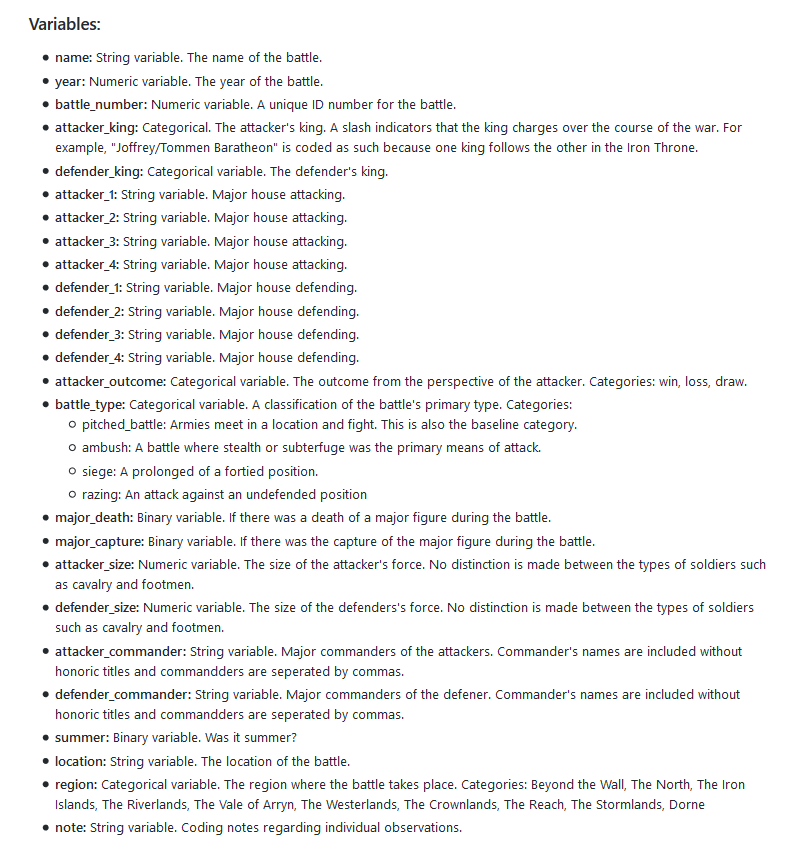
\includegraphics[totalheight=16cm]{battles.png}
\end{figure}

\pagebreak

\item Information about characters, when they died and a brief boi about the characters.\\
http://allendowney.blogspot.in/2015/03/bayesian-survival-analysis-for-game-of.html

Following is the schema of the data\\

\begin{figure}
\centering
        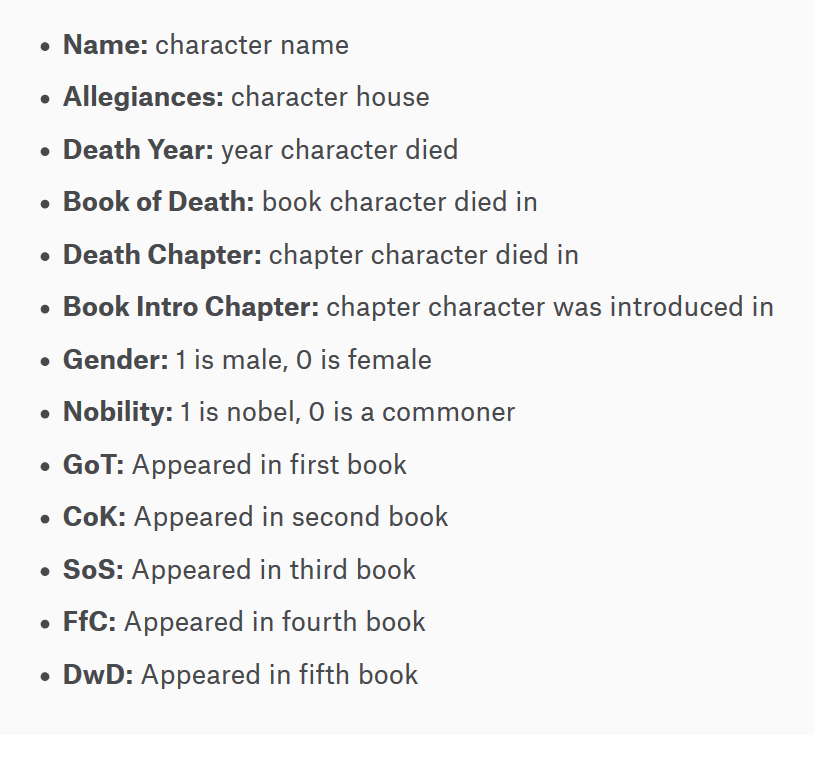
\includegraphics[totalheight=10cm]{deaths.png}
\end{figure}

\pagebreak

\item A collection of all the character predictions. This dataset contains an expanded view on character deaths, including predictions of how likely they are to die. (Prediction's come from A Song of Ice and Data's algorithm)\\
https://got.show/

\begin{figure}
\centering
        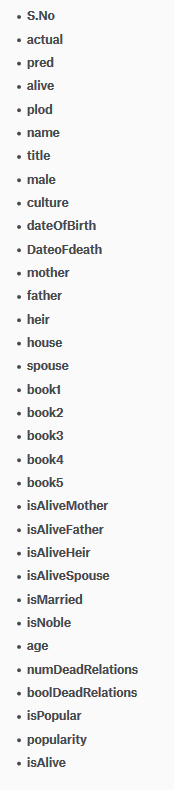
\includegraphics[totalheight=13cm]{prediction.png}
\end{figure}

\pagebreak

\end{itemize}

\vspace{25px}

A python script was written to cleanup the data, create the database, tables and load the data into the tables. 
\section{Functionality and Components}

The following are the four classes we intend to have in our project and a brief description of the purpose they serve.

\begin{itemize}

\item \textbf{Class Ball :}

\begin{flushleft}

The Class Ball has data members for storing the radius of the ball, colour of the ball, X, Y and Z co-ordinates of it's centre, X, Y and Z components of the velocity and whether it's selected or not. The mass of the ball is assumed to be proportional to the cube of it's radius. 
\\
The member functions of the class Ball include the set and get functions, a display function, a reshape function and functions to handle collisions.\\ The set and get functions are used to access the aforementioned data members and modify their values respectively. The display function is used to display the ball and the reshape function is used to handle the case when the window is resized by the user.\\
When an object of type ball is created, it is randomly assigned a centre, a radius, and a velocity. It is also ensured that the balls do not overlap at the time of creation.
\end{flushleft}

\item \textbf{Class Table :}

\begin{flushleft}

The Class Table has data members corresponding to the coordinates of the vertices of the cube/table. The member function display is used to display the cube/table and the function reshape is used to resize the table if the screen size is changed. It also has set and get functions.
\end{flushleft}


\item \textbf{Class ScreenSaver :}

\begin{flushleft}

An object of the Class ScreenSaver is created when the program starts executing. It creates $\mathcal{O}(n)$ (where, n is the number of balls entered at the time of execution) objects of the class Ball, $\mathcal{O}(n)$ pthreads, one to control the motion of each ball,$\mathcal{O}(n)$ mutex locks, a light source ( to give 3D appearance to the balls ) and one object of the class table. \\
\medskip

The class screensaver is the heart of the program and spans across three .cpp files. The files and their functionalities are :\\

\begin{itemize}

\item { \bf Handler :} 
The functions in this file take care of the operations that the user can perform on the screensaver through the GUI, Keyboard and Mouse. The list of the functionalities is provided in the README. The functions take requests from the user and call appropriate functions.

\item { \bf Initialization :}
The role of the functions in this file is to initialize the balls, the table, the lighting and the background. The initialization occurs when the program starts.There is also a function to destroy all the allocated memory and close the GUI windows when the program is terminated.

\item { \bf Render : }
The functions declared in this take care of the display sequences and reshapes that happen during the execution of the screensaver.  

\end{itemize}

\item \textbf{Class Menu :} 
This class contains some of the operations that the user can perform on the screensaver. It also handles the actions that happen 

\medskip
\medskip
\textbf{The subcomponents, segregated by functionality, are :}

\begin{itemize}

\item \textbf{GUI} : The GUI is handled by initializing an object of type screensaver that in turn creates the balls and the table and a menu which display themselves. The menu is created for the user to send requests and modify the appearance of the screensaver.

\item \textbf{Physics} : The physics is handled by the threads. The threads call a solver function which accepts as parameters velocities, masses and co-ordinates. It then returns the new velocities.

The following equations were solved to obtain 
\begin{equation}
\hat{n} = \frac{\vec{R_{1}} - \vec{R_{2}}}{ \parallel \vec{R_{1}} - \vec{R_{2}} \parallel}
\end{equation}
\begin{equation}
\vec{V_{1}^{'}} := \vec{V_{1}} + (\frac{m_{2}}{m_{1} + m_{2}}((1+e)\vec{V_{1}} - (1+e)\vec{V_{2}})\cdotp\hat{n})\hat{n}
\end{equation}
\begin{equation}
\vec{V_{2}^{'}} := \vec{V_{2}} + (\frac{m_{1}}{m_{1} + m_{2}}((1+e)\vec{V_{2}} - (1+e)\vec{V_{1}})\cdotp\hat{n})\hat{n}
\end{equation}


\item \textbf{Threading} : The updates of the co-ordinates and velocities of balls are handled by threads. They communicate through one to one communication, using message queue. Mutexes and conditional variables will be used appropriately.


\end{itemize}


\end{flushleft}

\end{itemize}

\section{Testing}

valgrind and gdb have to be used for testing. This is because of the threading involved. The components that require testing are :
\begin{itemize}


\item \textbf{Table :}
An object of type table would be created by using eight points to make the cube ( or four points to make a square ) and would then displayed on the window. Then the window then resized in order to check the correctness of the reshape member function. The feature of transition can be tested by actually testing the transition itself.

\item \textbf{Ball :}
The ball provides most of the functionality to our application. Hence we test it by testing various tiny portions. Following are the steps that we plan to take :

\begin{enumerate}

\item { Test the display functions - stationary, moving without thread, moving with threads }

\item { Collisions between the ball and the table would then be handled.}

\item { Switch to 3D. and repeat step 1 and 2.}

\item { Additional features such as selection can be tested as and when they are implemented. Modularity should allow us to implement the features without altering the already functioning code. }
\end{enumerate}
Floating point errors that happen during the execution of the program to be handled by varying the radius of the balls and handling corner cases.\\

\item { \bf Menu : }
Corresponding to each functionality that the screensaver provides, testing would be done for each of the operation the user can perform and corner cases would be handled. Following are some of the points that we plan to keep in mind :

\begin{enumerate}

\item { The user can increase the velocity of the ball only till a certain limit.}

\item { The number of balls in the screensaver, the user can have are bounded above. }

\item { The user can zoom- in and zoom-out till a certain point. }

\end{enumerate}

\item \textbf{Physics :} Since our physics part is a set of equations in a seperate function, we execute this function for a set of values to ensure that the output is correct, after which, we ensure that all corner-cases are handled.

\item \textbf{Memory Handling} : When the user sends a request to close the screensaver, all dynamically allocated memory is de-allocated and the GUI windows are closed. This is all done in the 'exitter' function which is called after the termination of 'glutmainloop()'. Valgrind will be used to ensure that there are no memory leaks i.e. to ensure that all dynamically allocated memory is released by the time the program is terminated. 

\item \textbf{Thread Synchronization} : Thread safety and possible race coditions will be tested using valgrind's helgrind.

\end{itemize}


\section{Sub-component Interaction}

\begin{flushleft}

The various sub-component interactions we have to consider are:
\begin{itemize}

\item \textbf{Inter Thread Communication :} \\ An entire section will be devoted to this.

\item \textbf{Collision between two Balls :}\\


\begin{flushleft}

If the distance between the centres of two balls is less than or equal to the sum of their radii then the collision condition for the two balls is satisfied else not. If there was a collision between two balls then the solveBallCollision function was called that took two objects of type Ball and computed their new velocities based on the equations of motion and assuming perfectly elastic collision.

\end{flushleft}


\item \textbf{Collision between a Ball and a Wall :} \\

\begin{flushleft}

In this type of collision the wall is assumed to have infinite mass.\\

If the perpendicular distance between the centre of the ball and the wall is less than the radius of the ball then this collision occours else not. This collison was also handled by the solveWallCollision function that took an object of type Ball as parameter and modified its velocity using the equations of motion and assuming perfectly elastic collision. An option to change the coefficient of restitution is provided.

\end{flushleft}  



\end{itemize}

\end{flushleft}


\section{Interthread Communication}

Interthread communication was initially done by barrier synchronization. It was then moved on to simulate a one-to-one communication method. \\
The communication was achieved by using a messageQueue/mailBox. Ours is called mailBox. Its a vector of a queue of messages. Every thread sends these messages to the other threads. Each of the thread processes its own mailbox and updates accordingly. The messages contain ball data.\\


\section{Ball Speed}

\begin{flushleft}

The X, Y and Z components of the velocity corresponding to each ball are to be stored in the  object of the class Ball and have to lie in a certain range. When a collision between two balls or between a ball and the wall occours, these parameters are modified in accordance with the equations derived from Newton's Laws of Motion.  
\\
The threads also ensure that the balls don't go faster than the maximum velocity which has been hardcoded. The maximum velocity constraint is present to ensure that the graphics look smooth.

\end{flushleft}

\section{Additional Features :}

\begin{flushleft} 

During the execution of the screensaver, the user is provided with the following options:

\begin{itemize}

\item { \bf 3D Mode :} The user has an option to switch between 2D and 3D modes. In the 3D mode, the balls move in a cube shaped wire frame.` 

\item { \bf Lighting :} A light source was placed in the screensaver so that the balls appear to be spheres and have a 3D appearance.

\item \textbf{Selection of a ball:}
The user is given the option of selecting a ball using the mouse ( \textbf{left mouse button click} ) or by using the \textbf{left and right arrow keys}. As soon as a ball is selected it's color changes to \textbf{White}. Once the desired ball has been selected, the following operations could be performed :

\begin{enumerate}

\item The user can increase the speed of the ball using the \textbf{up} arrow key. 

\item The user can decrease the speed of the ball by pressing the \textbf{down} arrow key.

\item The user can change the colour of the ball by pressing the 'C' character key.

\end{enumerate}

\item { \bf Starfield Background :}
In order to add an overall visual appeal to the screensaver, a starfield background was added. This was done by adding a texture using SDL to load the image.

\item { \bf Gravity and Coefficient of Restitution :} Gravity can be introduced by pressing the button available on the GUI window, or by using the 'G' key. All the balls are attracted towards a face of the cube and the coefficient of restitution between that face of the cube and the balls is set to a fixed value.

\item{ \bf Blink on Collision :}
Whenever a collision between two balls takes place, they were made to blink for a small amount of time.

\item{ \bf Pause and Exit :}
The user can pause/resume the screensaver by pressing 'Spacebar'. The screensaver can be closed by pressing the 'Escape' key.

\item \textbf{FullScreen Mode :}
The user can toggle between fullscreen and windowed modes by pressing the 'F' character key.

\item { \bf Change the resolution of the balls :}
The user can change the resolution of the balls during the execution of the screensaver. This would be done by changing the variables 'NUMSLICES' and 'NUMSTACKS' that the sphere takes while rendering. We intend to provide a few modes, which will act as a tribute to the creators.

\end{itemize}

\end{flushleft}

\end{document}